Con el fin de corroborar y ajustar los resultados teóricos obtenidos, se realiza la simulación del circuito mediante \texttt{SPICE Orcad}.

\Flor{Cambiar por el circuito actual, con C=330p}
\begin{figure}[H]
	\centering
	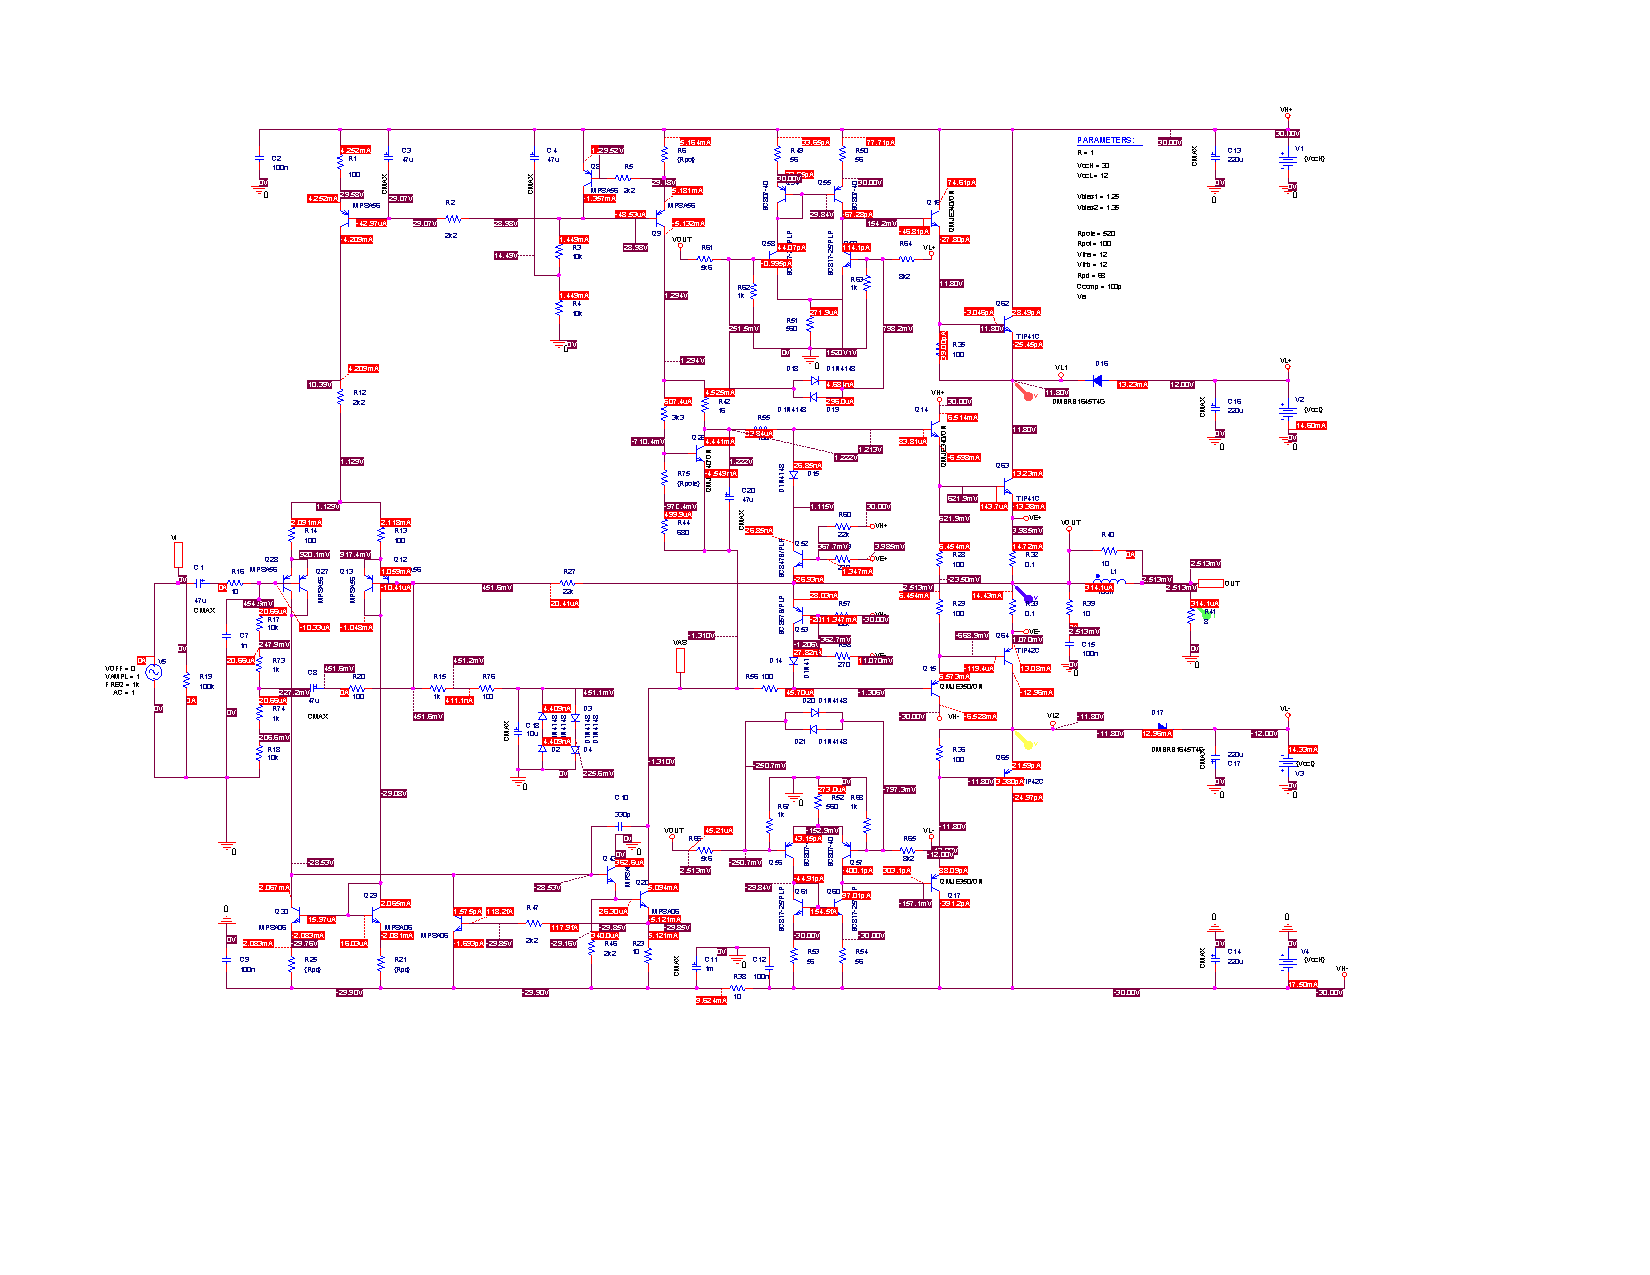
\includegraphics[scale=0.5]{sim_polarizacion.pdf}
	\caption{Tensiones y corrientes de reposo.}
	\label{fig:sim_pol}
\end{figure}


En la figura \ref{fig:sim_pol} se muestran las tensiones y corrientes en continua, siendo congruentes con los valores esperados.

